
\documentclass[10pt,aspectratio=169]{beamer}

%================================================
% Theme
%================================================
\usetheme[numbering=fraction,progressbar=frametitle]{metropolis}

%================================================
% Packages
%================================================
\usepackage{amsmath,amssymb}
\usepackage{booktabs}
\usepackage{tikz}
\usetikzlibrary{automata,positioning,arrows.meta,calc,trees}
\usepackage[useregional]{datetime2}
\usepackage{xcolor}
\usepackage{listings}

%================================================
% Metadata
%================================================
\newcommand{\LastCompiled}{\DTMnow}

\title{Theory of Computation}
\subtitle{Lecture 4: Nondeterminism and Nondeterministic Finite Automata}
\author{Sheikh Azizul Hakim\\Lecturer, Department of CSE, BUET}
\date{Last compiled: \LastCompiled}

%================================================
% Listings
%================================================
\lstdefinestyle{code}{
  basicstyle=\ttfamily\small,
  frame=single,
  backgroundcolor=\color{black!4},
  rulecolor=\color{black!20},
  showstringspaces=false,
  columns=fullflexible,
  keepspaces=true
}
\lstset{style=code}

%================================================
% Helpers
%================================================
\newcommand{\eps}{\varepsilon}
\newcommand{\powset}[1]{\mathcal P({#1})}
\newcommand{\lang}[1]{\mathsf{#1}}

\tikzset{
  every state/.style={minimum size=8mm},
  >=Stealth,
  shorten >=1pt,
}

%================================================
\begin{document}

%================================================
\maketitle

%================================================
\begin{frame}[standout]
Sometimes finding a solution is hard.

But verifying a guessed solution is easy.
\end{frame}

%================================================
\section{Lecture 4A: The Philosophy of Nondeterminism}

%------------------------------------------------
\begin{frame}{The Central Question}

In deterministic computation, every step is forced.

\[
(\text{current state},\text{input symbol})
\longrightarrow
\text{exactly one next state}
\]

\vspace{1em}

Today we ask:

\begin{center}
What if a machine could explore many possibilities?
\end{center}

\pause

This idea is called \textbf{nondeterminism}.

\end{frame}

%------------------------------------------------
\begin{frame}{Find versus Verify}

Many computational tasks have two versions.

\vspace{0.5em}

\begin{center}
\begin{tabular}{lll}
\toprule
\textbf{Problem} & \textbf{Find} & \textbf{Verify} \\
\midrule
Maze & Find a path & Check a given path \\
Sudoku & Solve puzzle & Check a completed board \\
Password & Discover password & Test a candidate password \\
SAT & Find assignment & Check a given assignment \\
Proof & Find proof & Check a written proof \\
\bottomrule
\end{tabular}
\end{center}

\vspace{0.7em}

\pause
The second task is often much easier.

\end{frame}

%------------------------------------------------
\begin{frame}{Example: Maze}

Task:

\begin{center}
Find a path from the entrance to the exit.
\end{center}

\vspace{1em}

This may require search.

\pause

\vspace{1em}

But if someone gives us a candidate path, we can quickly check:

\begin{itemize}
\item Does it start at the entrance?
\item Does every step follow a valid corridor?
\item Does it end at the exit?
\end{itemize}

\vspace{0.5em}

\pause
Finding and verifying are different kinds of computation.

\end{frame}

%------------------------------------------------
\begin{frame}{Example: Sudoku}

Finding a solution may be difficult.

\vspace{1em}

Verifying a completed board is straightforward:

\begin{itemize}
\item Check every row.
\item Check every column.
\item Check every block.
\end{itemize}

\vspace{1em}

\pause
This distinction will reappear later in complexity theory as a central theme.

\end{frame}

%------------------------------------------------
\begin{frame}{The Nondeterministic Dream}

Imagine a machine that can say:

\begin{quote}
Let me guess the correct branch of the search.
\end{quote}

\vspace{1em}

If the guess can be verified, the machine accepts.

\pause

\vspace{1em}

This is not how ordinary computers physically work.

But it is an extremely useful mathematical abstraction.

\end{frame}

%------------------------------------------------
\begin{frame}{Three Ways to Think About Nondeterminism}

\begin{enumerate}
\item \textbf{Magical guessing}

The machine guesses the correct choice.

\vspace{0.4em}

\item \textbf{Parallel universes}

All choices are explored simultaneously.

\vspace{0.4em}

\item \textbf{Computation tree}

The computation branches into many paths.
\end{enumerate}

\vspace{1em}

\pause
For finite automata, these viewpoints describe the same idea.

\end{frame}

%------------------------------------------------
\begin{frame}{Does Nondeterminism Exist Physically?}

Probably not as a literal machine that always guesses correctly.

\vspace{1em}

But theoretical computer science often studies idealized models.

\vspace{0.5em}

Examples:

\begin{itemize}
\item infinite tapes,
\item real numbers,
\item perfect randomness,
\item nondeterministic choices.
\end{itemize}

\vspace{0.5em}

\pause
Idealized models help us understand the structure and limits of computation.

\end{frame}

%------------------------------------------------
\begin{frame}{Why Study It Then?}

Nondeterminism models the shape of search.

\vspace{1em}

It appears behind many real computational tools:

\begin{itemize}
\item backtracking algorithms,
\item SAT solvers,
\item theorem provers,
\item symbolic execution,
\item program analysis,
\item AI planning,
\item regex engines.
\end{itemize}

\end{frame}

%------------------------------------------------
\begin{frame}[standout]
Nondeterminism is not merely an automata trick.

It is one of the central ideas of theoretical computer science.
\end{frame}

%================================================
\section{Lecture 4B: From DFA to NFA}

%------------------------------------------------
\begin{frame}{Recall: DFA}

A deterministic finite automaton has

\[
M=(Q,\Sigma,\delta,q_0,F).
\]

\vspace{1em}

The transition function is

\[
\delta:Q\times\Sigma\rightarrow Q.
\]

\vspace{1em}

For each state and input symbol, there is exactly one next state.

\end{frame}

%------------------------------------------------
\begin{frame}{What Changes in an NFA?}

In a nondeterministic finite automaton, one situation may have many possible next states.

\vspace{1em}

Instead of

\[
(q,a)\longmapsto q'
\]

we allow

\[
(q,a)\longmapsto \{q_1,q_2,\ldots,q_k\}.
\]

\vspace{1em}

The machine may branch.

\end{frame}

%------------------------------------------------
\begin{frame}{A First Language}

Let

\[
\lang{CONTAINS}_{101}
=
\{w\in\{0,1\}^*: w \text{ contains }101\text{ as a substring}\}.
\]

\vspace{1em}

Examples in the language:

\[
101,\quad 0101,\quad 1010,\quad 1110100.
\]

Examples not in the language:

\[
\eps,\quad 0,\quad 11,\quad 1000,\quad 0100.
\]

\end{frame}

%------------------------------------------------
\begin{frame}{DFA Thinking}

To recognize whether the input contains \(101\), a DFA keeps track of partial progress.

\vspace{1em}

It remembers whether it has recently seen:

\[
\text{nothing useful},\qquad 1,\qquad 10,\qquad 101.
\]

\vspace{1em}

This is perfectly possible.

\pause

But there is another way to think.

\end{frame}

%------------------------------------------------
\begin{frame}{NFA Thinking}

Whenever the machine sees a \(1\), it may guess:

\begin{center}
This \(1\) is the beginning of \(101\).
\end{center}

\vspace{1em}

If the guess is correct, one branch reaches an accepting state.

If the guess is wrong, that branch dies.

\vspace{1em}

\pause
The input is accepted if at least one guess succeeds.

\end{frame}

%------------------------------------------------
\begin{frame}{NFA for Strings Containing \(101\)}

\begin{center}
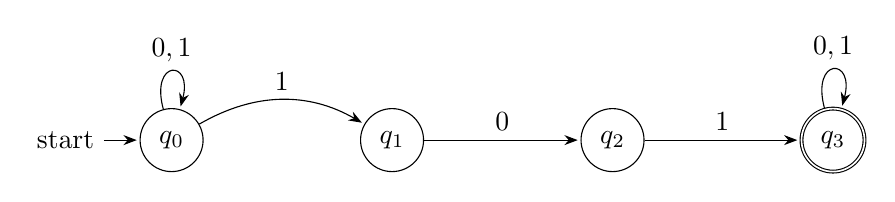
\begin{tikzpicture}[
->,
node distance=2.8cm,
every state/.style={minimum size=8mm}
]
\node[state,initial] (q0) {$q_0$};
\node[state,right of=q0] (q1) {$q_1$};
\node[state,right of=q1] (q2) {$q_2$};
\node[state,accepting,right of=q2] (q3) {$q_3$};

\path
(q0) edge[loop above] node{\(0,1\)} ()
(q0) edge[bend left] node[above]{\(1\)} (q1)
(q1) edge node[above]{\(0\)} (q2)
(q2) edge node[above]{\(1\)} (q3)
(q3) edge[loop above] node{\(0,1\)} ();
\end{tikzpicture}
\end{center}

\vspace{0.5em}

The branch \(q_0\to q_1\to q_2\to q_3\) verifies one guessed occurrence of \(101\).

\end{frame}
%------------------------------------------------
\begin{frame}{Three Outcomes of a Branch}

In an NFA, a single input may create many computation branches.

\vspace{0.7em}

A branch can end in three different ways:

\begin{center}
\begin{tabular}{ll}
\toprule
\textbf{Outcome} & \textbf{Meaning}\\
\midrule
\textcolor{green!50!black}{Accepted} & input is fully read and the branch ends in an accepting state\\
\textcolor{red!70!black}{Rejected} & input is fully read but the branch ends in a non-accepting state\\
\textcolor{gray!70!black}{Dead} & the branch gets stuck before the input is fully read\\
\bottomrule
\end{tabular}
\end{center}

\vspace{0.7em}

\pause
The NFA accepts the input if \textbf{at least one} branch is accepted.

\end{frame}

%------------------------------------------------
\begin{frame}{Why Is This Nondeterministic?}

At state \(q_0\), on input \(1\), the machine has two choices:

\[
\delta(q_0,1)=\{q_0,q_1\}.
\]

\vspace{0.7em}

Interpretation:

\begin{itemize}
\item \(q_0\): ignore this \(1\);
\item \(q_1\): guess this \(1\) starts the pattern \(101\).
\end{itemize}

\vspace{0.7em}

\pause
Both possibilities are explored as separate branches.

\end{frame}

%------------------------------------------------
\begin{frame}{Computation Tree for \(0101\)}

\small
Input: \(0101\)

\begin{center}
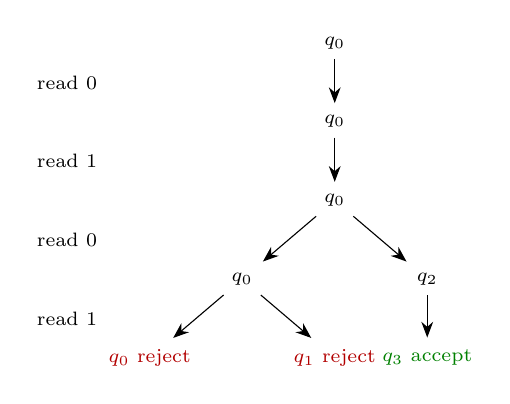
\begin{tikzpicture}[
  level distance=1.0cm,
  sibling distance=2.35cm,
  every node/.style={font=\scriptsize},
  edge from parent/.style={draw,-{Stealth[length=2mm]}}
]
\node {\(q_0\)}
  child { node {\(q_0\)}
    child { node {\(q_0\)}
      child { node {\(q_0\)}
        child { node[text=red!70!black] {\(q_0\) reject} }
        child { node[text=red!70!black] {\(q_1\) reject} }
      }
      child { node {\(q_2\)}
        child { node[text=green!50!black] {\(q_3\) accept} }
      }
    }
  };

\node[font=\scriptsize] at (-3.4,-0.5) {read \(0\)};
\node[font=\scriptsize] at (-3.4,-1.5) {read \(1\)};
\node[font=\scriptsize] at (-3.4,-2.5) {read \(0\)};
\node[font=\scriptsize] at (-3.4,-3.5) {read \(1\)};
\end{tikzpicture}
\end{center}

\vspace{0.3em}

One leaf reaches \(q_3\in F\), so \(0101\) is accepted.

\end{frame}

%------------------------------------------------
\begin{frame}{Computation Tree for \(1000\)}

\small
Input: \(1000\)

\begin{center}
\begin{tikzpicture}[
  level distance=1.0cm,
  sibling distance=2.4cm,
  every node/.style={font=\scriptsize},
  edge from parent/.style={draw,-{Stealth[length=2mm]}}
]
\node {\(q_0\)}
  child { node {\(q_0\)}
    child { node {\(q_0\)}
      child { node {\(q_0\)}
        child { node[text=red!70!black] {\(q_0\) reject} }
      }
    }
  }
  child { node {\(q_1\)}
    child { node {\(q_2\)}
      child { node[text=gray!70!black] {dead} }
    }
  };

\node[font=\scriptsize] at (-3.4,-0.5) {read \(1\)};
\node[font=\scriptsize] at (-3.4,-1.5) {read \(0\)};
\node[font=\scriptsize] at (-3.4,-2.5) {read \(0\)};
\node[font=\scriptsize] at (-3.4,-3.5) {read \(0\)};
\end{tikzpicture}
\end{center}

\vspace{0.3em}

The guessed \(101\)-branch dies at \(q_2\) on input \(0\).  
The surviving branch ends at non-accepting \(q_0\). So \(1000\) is rejected.

\end{frame}

%------------------------------------------------
\begin{frame}{Acceptance in an NFA}

Important rule:

\vspace{0.8em}

\begin{center}
\textbf{An NFA accepts if at least one computation branch accepts.}
\end{center}

\vspace{0.8em}

\begin{itemize}
\item Accepted branch: input consumed, final state is in \(F\).
\item Rejected branch: input consumed, final state is not in \(F\).
\item Dead branch: no valid transition before the input is consumed.
\end{itemize}

\vspace{0.5em}

\pause
Many bad branches do not matter if one good branch accepts.

\end{frame}

%------------------------------------------------
\begin{frame}{Proving Acceptance versus Rejection}

To show that an NFA \textbf{accepts} a string, it is enough to show one accepting branch.

\vspace{0.7em}

\begin{center}
\begin{tabular}{ll}
\toprule
\textbf{Claim} & \textbf{What must be shown?}\\
\midrule
\(w\) is accepted & exhibit one valid accepting branch\\
\(w\) is rejected & rule out every possible accepting branch\\
\bottomrule
\end{tabular}
\end{center}

\vspace{0.8em}

\pause

This is the ``magical guessing'' viewpoint:

\begin{center}
If an accepting branch exists, the NFA may guess that branch.
\end{center}

\vspace{0.6em}

\pause

But for rejection, there is no shortcut:

\begin{center}
Every branch must be checked, and none may accept.
\end{center}

\end{frame}
%------------------------------------------------
\begin{frame}[standout]
A DFA has one timeline.

An NFA has many possible timelines.
\end{frame}


%------------------------------------------------
\begin{frame}{Formal Definition}

A nondeterministic finite automaton is a 5-tuple

\[
M=(Q,\Sigma,\delta,q_0,F),
\]

where:

\begin{itemize}
\item \(Q\) is a finite set of states,
\item \(\Sigma\) is the input alphabet,
\item \(q_0\in Q\) is the start state,
\item \(F\subseteq Q\) is the set of accepting states,
\item $\delta:Q\times\Sigma\rightarrow \powset{Q}$ is the transition function.
\end{itemize}

\vspace{0.5em}

\textbf{Only \(\delta\) differs from the DFA case.}

\end{frame}

%------------------------------------------------
\begin{frame}{DFA versus NFA Transition Functions}

For a DFA:

\[
\delta:Q\times\Sigma\rightarrow Q.
\]

For an NFA:

\[
\delta:Q\times\Sigma\rightarrow \powset{Q}.
\]

\vspace{1em}

Here \(\powset{Q}\) means the set of all subsets of \(Q\).

\end{frame}

%------------------------------------------------
\begin{frame}{Why a Set of States?}

Suppose

\[
Q=\{q_0,q_1,q_2\}.
\]

Then

\[
\powset{Q}
=
\{
\emptyset,
\{q_0\},
\{q_1\},
\{q_2\},
\{q_0,q_1\},
\{q_0,q_2\},
\{q_1,q_2\},
\{q_0,q_1,q_2\}
\}.
\]

\vspace{0.5em}

An NFA transition may return any one of these subsets.

\end{frame}

%------------------------------------------------
\begin{frame}{Interpreting the Output of \(\delta\)}

\[
\delta(q,a)=\emptyset
\]

means no branch survives.

\vspace{1em}

\[
\delta(q,a)=\{r\}
\]

means exactly one next possibility.

\vspace{1em}

\[
\delta(q,a)=\{r,s,t\}
\]

means the computation branches into three possibilities.

\end{frame}

%------------------------------------------------
\begin{frame}{Formal Specification of the \(101\) NFA}

\[
Q=\{q_0,q_1,q_2,q_3\},
\qquad
\Sigma=\{0,1\},
\qquad
F=\{q_3\}.
\]

\[
q_0 \text{ is the start state.}
\]

\vspace{1em}

The transition function is:

\[
\begin{array}{c|cc}
\delta & 0 & 1\\
\hline
q_0 & \{q_0\} & \{q_0,q_1\}\\
q_1 & \{q_2\} & \emptyset\\
q_2 & \emptyset & \{q_3\}\\
q_3 & \{q_3\} & \{q_3\}
\end{array}
\]

\end{frame}

%------------------------------------------------
\begin{frame}{Notice the Difference}

In a DFA table, each entry is a state.

\[
q_0,\quad q_1,\quad q_2
\]

\vspace{1em}

In an NFA table, each entry is a set of states.

\[
\emptyset,\quad \{q_0\},\quad \{q_0,q_1\}
\]

\vspace{1em}

The table is just a precise way to define the transition function.

\end{frame}

%------------------------------------------------
\begin{frame}{Every DFA Is an NFA}

A DFA transition

\[
\delta(q,a)=r
\]

can be viewed as the NFA transition

\[
\delta(q,a)=\{r\}.
\]

\vspace{1em}

So every DFA is automatically an NFA.

\pause

\vspace{1em}

But is every NFA equivalent to some DFA?

That is the big question.

\end{frame}

%================================================
\section{Lecture 4C: More Examples}

%------------------------------------------------
\begin{frame}{Example 1: Contains \texttt{fed} or \texttt{dff}}

Language over $\Sigma=\{d,e,f\}$:
\[
L=\{w\in\{d,e,f\}^*: w\text{ contains }fed\text{ or }dff\text{ as a substring}\}.
\]

\[
\text{Members: } fed,\ dff,\ efed,\ dffd,\ ffdff
\]

\[
\text{Non-members: } \eps,\ d,\ ff,\ def,\ fef,\ edf
\]

\vspace{0.5em}

\pause
The NFA guesses where one of the two target substrings begins.

\end{frame}

%------------------------------------------------
\begin{frame}{NFA Idea: Two Possible Patterns}

We want to detect either

\[
fed
\qquad\text{or}\qquad
dff.
\]

\vspace{0.7em}

The machine scans the input in state $q_0$.

\begin{itemize}
\item When it sees $f$, it may guess that $fed$ is beginning.
\item When it sees $d$, it may guess that $dff$ is beginning.
\end{itemize}

\vspace{0.7em}

\pause
If either guessed pattern is completed, the input is accepted.

\end{frame}

%------------------------------------------------
\begin{frame}{NFA for Contains \texttt{fed} or \texttt{dff}}

\begin{center}
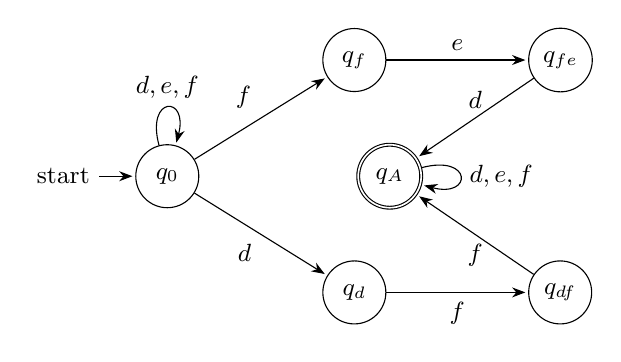
\begin{tikzpicture}[
  ->,>=Stealth,shorten >=1pt,
  node distance=2.05cm,
  every state/.style={minimum size=8mm},
  every node/.style={font=\small}
]

\node[state,initial] (q0) {$q_0$};

\node[state,above right=0.9cm and 1.8cm of q0] (qf) {$q_f$};
\node[state,right=1.8cm of qf] (qfe) {$q_{fe}$};

\node[state,below right=0.9cm and 1.8cm of q0] (qd) {$q_d$};
\node[state,right=1.8cm of qd] (qdf) {$q_{df}$};

\node[state,accepting,right=2.0cm of q0] (A) {$q_A$};

\path
(q0) edge[loop above] node {$d,e,f$} ()
(q0) edge node[above left] {$f$} (qf)
(q0) edge node[below left] {$d$} (qd)

(qf) edge node[above] {$e$} (qfe)
(qfe) edge node[above] {$d$} (A)

(qd) edge node[below] {$f$} (qdf)
(qdf) edge node[below] {$f$} (A)

(A) edge[loop right] node {$d,e,f$} ();

\end{tikzpicture}
\end{center}

\vspace{0.3em}
\small Missing transitions mean that the corresponding branch dies.

\end{frame}

%------------------------------------------------
\begin{frame}{Example 2: Guessing a Split Point}

Language over $\Sigma=\{a,b\}$:
\[
L=\{w_1w_2 : |w_1|\text{ is a multiple of } 3
\text{ and } w_2\text{ has an even number of }b\text{'s}\}.
\]

\[
w_1w_2 \text{ means the concatenation of } w_1 \text{ and } w_2
\]

\[
\text{Members: } \eps,\ a,\ aa,\ bb,\ aaa,\ aab,\ abba
\]

\[
\text{Non-members: } b,\ ab,\ ba,\ aaab,\ abbb
\]

\vspace{0.5em}

\pause
The NFA guesses the split point, but without using an $\eps$-transition.

\end{frame}

%------------------------------------------------
\begin{frame}{The Intuition}

The top part tracks the length of the prefix modulo \(3\):

\[
r_0,\quad r_1,\quad r_2.
\]

\vspace{0.7em}

A split is allowed only when the prefix length is a multiple of \(3\), that is, at \(r_0\).

\vspace{0.7em}

\pause

From \(r_0\), on the next symbol, the NFA has two choices:

\begin{itemize}
\item keep reading \(w_1\);
\item treat this symbol as the first symbol of \(w_2\).
\end{itemize}

\end{frame}

%------------------------------------------------
\begin{frame}{NFA for Guessing the Split Point}

\begin{center}
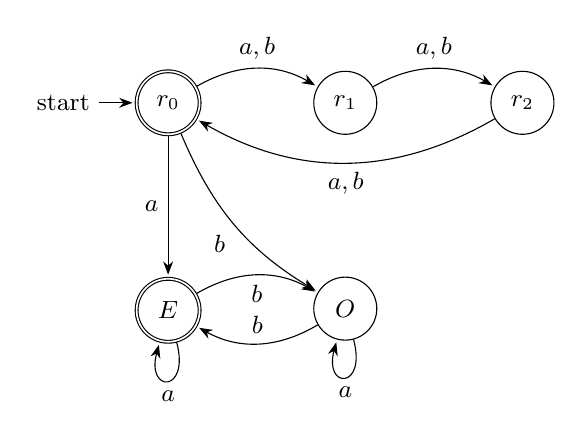
\begin{tikzpicture}[
  ->,>=Stealth,shorten >=1pt,
  node distance=2.25cm,
  every state/.style={minimum size=8mm},
  every node/.style={font=\small}
]

\node[state,initial,accepting] (r0) {$r_0$};
\node[state,right of=r0] (r1) {$r_1$};
\node[state,right of=r1] (r2) {$r_2$};

\node[state,accepting,below=1.8cm of r0] (E) {$E$};
\node[state,below=1.8cm of r1] (O) {$O$};

\path
(r0) edge[bend left] node[above] {$a,b$} (r1)
(r1) edge[bend left] node[above] {$a,b$} (r2)
(r2) edge[bend left] node[below] {$a,b$} (r0)

(r0) edge node[left] {$a$} (E)
(r0) edge[bend right=18] node[below left] {$b$} (O)

(E) edge[loop below] node {$a$} ()
(E) edge[bend left] node[below] {$b$} (O)
(O) edge[loop below] node {$a$} ()
(O) edge[bend left] node[above] {$b$} (E);

\end{tikzpicture}
\end{center}

\vspace{0.3em}
\small State \(r_0\) is accepting because the NFA may choose \(w_2=\eps\).

\end{frame}

%------------------------------------------------
\begin{frame}{Reading the Split-Point NFA}

The states \(r_0,r_1,r_2\) track

\[
|w_1| \bmod 3.
\]

\vspace{0.7em}

The states \(E,O\) track whether the guessed suffix \(w_2\) has an even or odd number of \(b\)'s.

\vspace{0.7em}

\pause

At \(r_0\), the NFA may begin reading \(w_2\):

\[
r_0 \xrightarrow{a} E,
\qquad
r_0 \xrightarrow{b} O.
\]

\vspace{0.5em}

No $\eps$-transition is used.

\end{frame}

%------------------------------------------------
\begin{frame}{Example 3: Missing at Least One Symbol}

Language over $\Sigma=\{a,b,c\}$:
\[
L=\{w\in\{a,b,c\}^*: w\text{ is missing at least one of }a,b,c\}.
\]

\[
\text{Members: } \eps,\ a,\ ab,\ bbbb,\ acac,\ ccaa
\]

\[
\text{Non-members: } abc,\ acb,\ baac,\ cbabc
\]

\vspace{0.5em}

\pause
The NFA guesses which symbol will be missing.

\end{frame}

%------------------------------------------------
\begin{frame}{NFA Idea: Guess the Missing Symbol}

The string is in the language if

\[
\text{it has no }a
\quad\text{or}\quad
\text{it has no }b
\quad\text{or}\quad
\text{it has no }c.
\]

\vspace{0.7em}

The NFA branches into three possible checks:

\[
q_{\neg a},\qquad q_{\neg b},\qquad q_{\neg c}.
\]

\vspace{0.7em}

\pause
Without $\eps$-transitions, the branching happens while reading the first input symbol.

\end{frame}

%------------------------------------------------
\begin{frame}{NFA for Missing at Least One Symbol}

\begin{center}
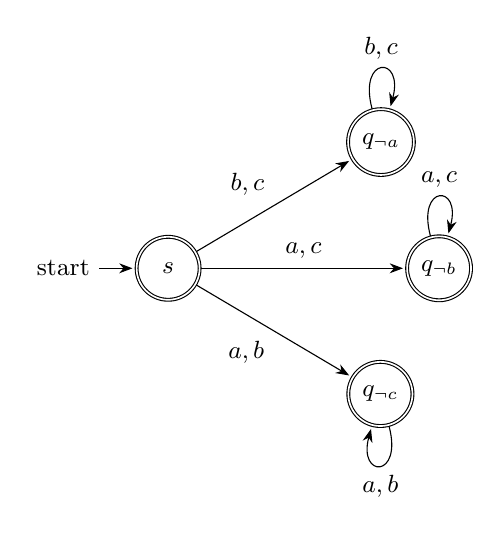
\begin{tikzpicture}[
  ->,>=Stealth,shorten >=1pt,
  node distance=2.4cm,
  every state/.style={minimum size=8mm},
  every node/.style={font=\small}
]

\node[state,initial,accepting] (s) {$s$};

\node[state,accepting,above right=1.0cm and 2.1cm of s] (noa) {$q_{\neg a}$};
\node[state,accepting,right=2.6cm of s] (nob) {$q_{\neg b}$};
\node[state,accepting,below right=1.0cm and 2.1cm of s] (noc) {$q_{\neg c}$};

\path
(s) edge node[above left] {$b,c$} (noa)
(s) edge node[above] {$a,c$} (nob)
(s) edge node[below left] {$a,b$} (noc)

(noa) edge[loop above] node {$b,c$} ()
(nob) edge[loop above] node {$a,c$} ()
(noc) edge[loop below] node {$a,b$} ();

\end{tikzpicture}
\end{center}

\vspace{0.3em}
\small State \(s\) accepts \(\eps\). A branch dies if it reads the symbol it guessed would be missing.

\end{frame}

%------------------------------------------------
\begin{frame}{Transition Table for the Missing-Symbol NFA}

\small
All four states shown here are accepting.

\begin{center}
\begin{tabular}{c|ccc}
\toprule
\textbf{State} & \textbf{on $a$} & \textbf{on $b$} & \textbf{on $c$}\\
\midrule
$s$ & $\{q_{\neg b},q_{\neg c}\}$ & $\{q_{\neg a},q_{\neg c}\}$ & $\{q_{\neg a},q_{\neg b}\}$\\
$q_{\neg a}$ & $\emptyset$ & $\{q_{\neg a}\}$ & $\{q_{\neg a}\}$\\
$q_{\neg b}$ & $\{q_{\neg b}\}$ & $\emptyset$ & $\{q_{\neg b}\}$\\
$q_{\neg c}$ & $\{q_{\neg c}\}$ & $\{q_{\neg c}\}$ & $\emptyset$\\
\bottomrule
\end{tabular}
\end{center}

\vspace{0.5em}

For example, on input \(abc\), every branch eventually dies.

\end{frame}

%------------------------------------------------
\begin{frame}{What These Examples Show}

\begin{itemize}
\item For substring search, an NFA guesses where the pattern begins.
\item For split languages, an NFA guesses where one part ends and the next begins.
\item For missing-symbol languages, an NFA guesses which condition will remain true.
\end{itemize}

\vspace{0.8em}

\pause

The common theme:

\begin{center}
\textbf{An NFA is good at expressing ``there exists a good choice.''}
\end{center}

\end{frame}
%================================================
\section{Lecture 4D: Epsilon Transitions}

%------------------------------------------------
\begin{frame}{Epsilon-NFA}

An \textbf{epsilon-NFA} is an NFA that may move without reading input.

\vspace{0.7em}

Formally, it is a 5-tuple
\[
M=(Q,\Sigma,\delta,q_0,F),
\]
where
\[
\delta:Q\times\Sigma_{\eps}\rightarrow \mathcal P(Q),
\qquad
\Sigma_{\eps}=\Sigma\cup\{\eps\}.
\]

\vspace{0.7em}

So a transition may be labeled by an ordinary input symbol, or by \(\eps\).

\[
q \xrightarrow{\eps} r
\]

means: move from \(q\) to \(r\) without consuming any input.

\end{frame}

%------------------------------------------------
\begin{frame}{How Does an Epsilon-NFA Accept?}

Let \(w\in\Sigma^*\). An epsilon-NFA accepts \(w\) if there exists a path

\[
q_0=p_0 \rightarrow p_1 \rightarrow \cdots \rightarrow p_m
\]

such that:

\begin{enumerate}
\item each transition label is either a symbol from \(\Sigma\) or \(\eps\);
\item after deleting all \(\eps\)'s from the labels, the remaining string is exactly \(w\);
\item the final state is accepting: \(p_m\in F\).
\end{enumerate}

\vspace{0.7em}

\pause
In short:

\begin{center}
\textbf{The machine may take free \(\eps\)-moves before, between, or after reading symbols.}
\end{center}

\end{frame}

%------------------------------------------------
\begin{frame}{Why \(\eps\)-Transitions Are Useful}

They make automata modular.

\vspace{0.8em}

Suppose we want to recognize

\[
L=\{ab,\ acd\}.
\]

\vspace{0.8em}

Both strings begin with \(a\). After reading \(a\), the machine must choose:

\[
\text{finish with } b
\qquad\text{or}\qquad
\text{finish with } cd.
\]

\vspace{0.8em}

With \(\eps\)-transitions, we can first read the common prefix \(a\), then freely jump into the appropriate suffix module.

\end{frame}

%------------------------------------------------
\begin{frame}{Epsilon-NFA for \(\{ab, acd\}\)}

\begin{center}
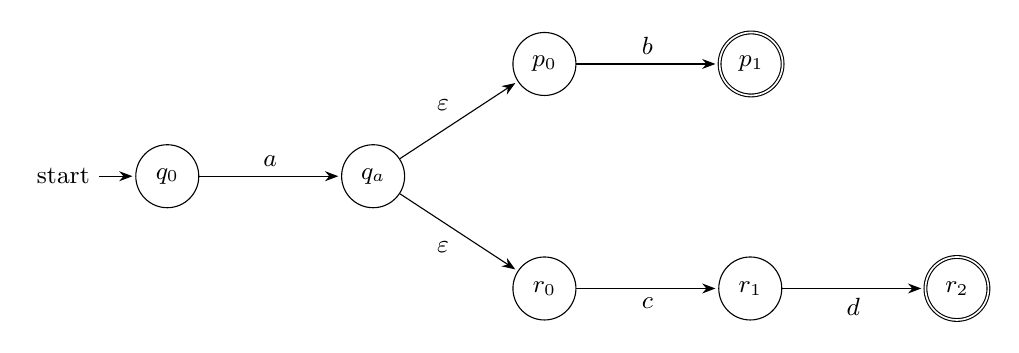
\begin{tikzpicture}[
  ->,>=Stealth,shorten >=1pt,
  node distance=2.0cm,
  every state/.style={minimum size=8mm},
  every node/.style={font=\small}
]

\node[state,initial] (q0) {$q_0$};
\node[state,right=1.8cm of q0] (qa) {$q_a$};

\node[state,above right=0.85cm and 1.6cm of qa] (p0) {$p_0$};
\node[state,accepting,right=1.8cm of p0] (p1) {$p_1$};

\node[state,below right=0.85cm and 1.6cm of qa] (r0) {$r_0$};
\node[state,right=1.8cm of r0] (r1) {$r_1$};
\node[state,accepting,right=1.8cm of r1] (r2) {$r_2$};

\path
(q0) edge node[above] {$a$} (qa)

(qa) edge node[above left] {$\eps$} (p0)
(qa) edge node[below left] {$\eps$} (r0)

(p0) edge node[above] {$b$} (p1)

(r0) edge node[below] {$c$} (r1)
(r1) edge node[below] {$d$} (r2);

\end{tikzpicture}
\end{center}

\vspace{0.4em}

The \(\eps\)-moves occur after the input symbol \(a\) has already been consumed.

\end{frame}

%------------------------------------------------
\begin{frame}{Computation Tree on Input \(acd\)}

\small
Input: \(acd\)

\begin{center}
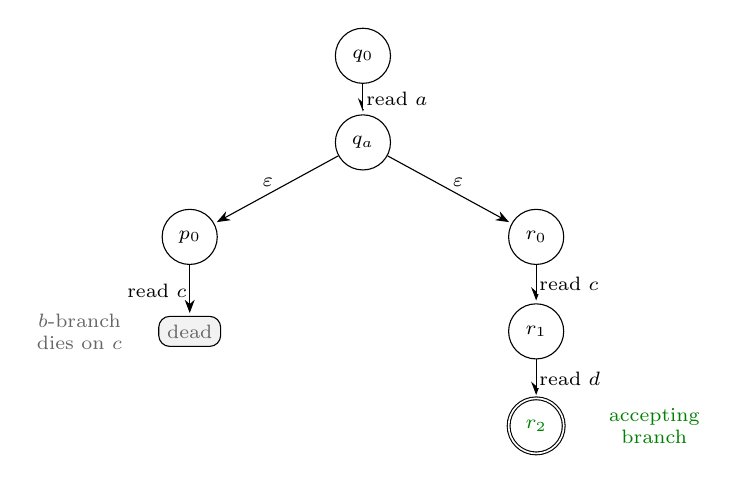
\begin{tikzpicture}[
  ->,>=Stealth,
  every node/.style={font=\scriptsize},
  st/.style={draw,circle,minimum size=7mm,inner sep=1pt},
  acc/.style={st,double,text=green!50!black},
  dead/.style={draw,rounded corners,fill=black!5,text=gray!80!black,
               inner sep=3pt},
  lab/.style={fill=white,inner sep=1pt,font=\scriptsize}
]

\node[st] (q0) at (0,0) {$q_0$};
\node[st] (qa) at (0,-1.1) {$q_a$};

\node[st] (p0) at (-2.2,-2.3) {$p_0$};
\node[dead] (pd) at (-2.2,-3.5) {dead};

\node[st] (r0) at (2.2,-2.3) {$r_0$};
\node[st] (r1) at (2.2,-3.5) {$r_1$};
\node[acc] (r2) at (2.2,-4.7) {$r_2$};

\draw (q0) -- node[lab,right] {read \(a\)} (qa);

\draw (qa) -- node[lab,above left] {\(\eps\)} (p0);
\draw (qa) -- node[lab,above right] {\(\eps\)} (r0);

\draw (p0) -- node[lab,left] {read \(c\)} (pd);

\draw (r0) -- node[lab,right] {read \(c\)} (r1);
\draw (r1) -- node[lab,right] {read \(d\)} (r2);

\node[text=gray!80!black,align=center] at (-3.6,-3.5)
  {\(b\)-branch\\dies on \(c\)};

\node[text=green!50!black,align=center] at (3.7,-4.7)
  {accepting\\branch};

\end{tikzpicture}
\end{center}
\vspace{0.4em}

The \(b\)-suffix branch dies on \(c\), but the \(cd\)-suffix branch accepts.

\end{frame}

%------------------------------------------------
\begin{frame}{One Accepting Computation Path}

For input \(acd\), one accepting path is:

\[
q_0
\xrightarrow{a}
q_a
\xrightarrow{\eps}
r_0
\xrightarrow{c}
r_1
\xrightarrow{d}
r_2.
\]

\vspace{0.8em}

After deleting the \(\eps\)-label, the consumed input is

\[
acd.
\]

\vspace{0.8em}

Since \(r_2\in F\), this path accepts. Therefore, the epsilon-NFA accepts \(acd\).

\end{frame}
%------------------------------------------------
\begin{frame}{A More Complex Epsilon-NFA: Accepted Case}

\small
Input for the computation tree: \(01011\)

\begin{center}
\begin{tikzpicture}[
  ->,>=Stealth,shorten >=1pt,
  node distance=1.55cm,
  every state/.style={minimum size=7mm},
  every node/.style={font=\scriptsize}
]

\node[state,initial] (s) {$s$};
\node[state,above right=0.55cm and 1.2cm of s] (a0) {$a_0$};
\node[state,below right=0.55cm and 1.2cm of s] (b0) {$b_0$};

\node[state,right=1.35cm of a0] (a1) {$a_1$};
\node[state,right=1.35cm of a1] (a2) {$a_2$};
\node[state,right=1.35cm of a2] (a3) {$a_3$};
\node[state,accepting,right=1.35cm of a3] (f) {$f$};

\node[state,right=1.35cm of b0] (b1) {$b_1$};
\node[state,right=1.35cm of b1] (b2) {$b_2$};

\path
(s) edge node[above left] {$\eps$} (a0)
(s) edge node[below left] {$\eps$} (b0)

(a0) edge node[above] {$0$} (a1)
(a1) edge[loop above] node {$1$} ()
(a1) edge node[above] {$0$} (a2)
(a2) edge node[above] {$1$} (a3)
(a3) edge node[above] {$1$} (f)

(b0) edge[loop below] node {$0$} ()
(b0) edge node[below] {$1$} (b1)
(b1) edge node[below] {$0$} (b2);

\end{tikzpicture}
\end{center}

\vspace{0.3em}
The upper module tries to read \(01^*011\). The lower module is a tempting branch, but it will die on this input.

\end{frame}

%------------------------------------------------
\begin{frame}{Entire Computation Tree: \(01011\)}

\scriptsize
\begin{center}
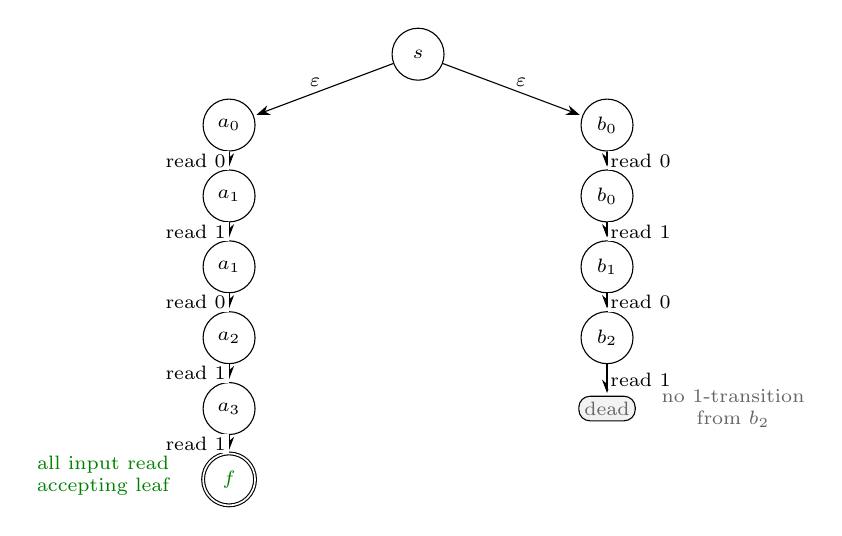
\begin{tikzpicture}[
  ->,>=Stealth,
  every node/.style={font=\scriptsize},
  st/.style={draw,circle,minimum size=6.6mm,inner sep=1pt},
  acc/.style={st,double,text=green!50!black},
  dead/.style={draw,rounded corners,fill=black!5,text=gray!80!black,inner sep=2pt},
  lab/.style={fill=white,inner sep=1pt,font=\scriptsize}
]

\node[st] (s) at (0,0) {$s$};

\node[st] (a0) at (-2.4,-0.9) {$a_0$};
\node[st] (b0) at (2.4,-0.9) {$b_0$};

\node[st] (a1) at (-2.4,-1.8) {$a_1$};
\node[st] (b0b) at (2.4,-1.8) {$b_0$};

\node[st] (a1b) at (-2.4,-2.7) {$a_1$};
\node[st] (b1) at (2.4,-2.7) {$b_1$};

\node[st] (a2) at (-2.4,-3.6) {$a_2$};
\node[st] (b2) at (2.4,-3.6) {$b_2$};

\node[st] (a3) at (-2.4,-4.5) {$a_3$};
\node[dead] (bd) at (2.4,-4.5) {dead};

\node[acc] (f) at (-2.4,-5.4) {$f$};

\draw (s) -- node[lab,above left] {$\eps$} (a0);
\draw (s) -- node[lab,above right] {$\eps$} (b0);

\draw (a0) -- node[lab,left] {read \(0\)} (a1);
\draw (b0) -- node[lab,right] {read \(0\)} (b0b);

\draw (a1) -- node[lab,left] {read \(1\)} (a1b);
\draw (b0b) -- node[lab,right] {read \(1\)} (b1);

\draw (a1b) -- node[lab,left] {read \(0\)} (a2);
\draw (b1) -- node[lab,right] {read \(0\)} (b2);

\draw (a2) -- node[lab,left] {read \(1\)} (a3);
\draw (b2) -- node[lab,right] {read \(1\)} (bd);

\draw (a3) -- node[lab,left] {read \(1\)} (f);

\node[text=green!50!black,align=center] at (-4.0,-5.35)
  {all input read\\accepting leaf};
\node[text=gray!80!black,align=center] at (4.0,-4.5)
  {no \(1\)-transition\\from \(b_2\)};

\end{tikzpicture}
\end{center}

\vspace{0.2em}
The input is accepted because at least one branch consumes all five symbols and ends in \(f\).

\end{frame}

%------------------------------------------------
\begin{frame}{A More Complex Epsilon-NFA: Rejected Case}

\small
Input for the computation tree: \(10100\)

\begin{center}
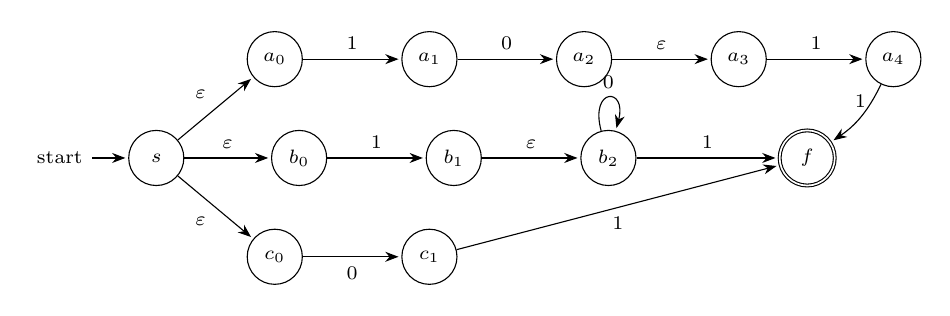
\begin{tikzpicture}[
  ->,>=Stealth,shorten >=1pt,
  node distance=1.45cm,
  every state/.style={minimum size=7mm},
  every node/.style={font=\scriptsize}
]

\node[state,initial] (s) {$s$};
\node[state,above right=0.75cm and 1.0cm of s] (a0) {$a_0$};
\node[state,right=1.1cm of s] (b0) {$b_0$};
\node[state,below right=0.75cm and 1.0cm of s] (c0) {$c_0$};

\node[state,right=1.25cm of a0] (a1) {$a_1$};
\node[state,right=1.25cm of a1] (a2) {$a_2$};
\node[state,right=1.25cm of a2] (a3) {$a_3$};
\node[state,right=1.25cm of a3] (a4) {$a_4$};

\node[state,right=1.25cm of b0] (b1) {$b_1$};
\node[state,right=1.25cm of b1] (b2) {$b_2$};

\node[state,right=1.25cm of c0] (c1) {$c_1$};
\node[state,accepting,right=1.8cm of b2] (f) {$f$};

\path
(s) edge node[above left] {$\eps$} (a0)
(s) edge node[above] {$\eps$} (b0)
(s) edge node[below left] {$\eps$} (c0)

(a0) edge node[above] {$1$} (a1)
(a1) edge node[above] {$0$} (a2)
(a2) edge node[above] {$\eps$} (a3)
(a3) edge node[above] {$1$} (a4)
(a4) edge[bend left=15] node[above] {$1$} (f)

(b0) edge node[above] {$1$} (b1)
(b1) edge node[above] {$\eps$} (b2)
(b2) edge[loop above] node {$0$} ()
(b2) edge node[above] {$1$} (f)

(c0) edge node[below] {$0$} (c1)
(c1) edge node[below] {$1$} (f);

\end{tikzpicture}
\end{center}

\vspace{0.2em}
This machine has three \(\eps\)-chosen modules, but none can consume all of \(10100\) and finish accepting.

\end{frame}

%------------------------------------------------
\begin{frame}{Entire Computation Tree: \(10100\)}

\scriptsize
\begin{center}
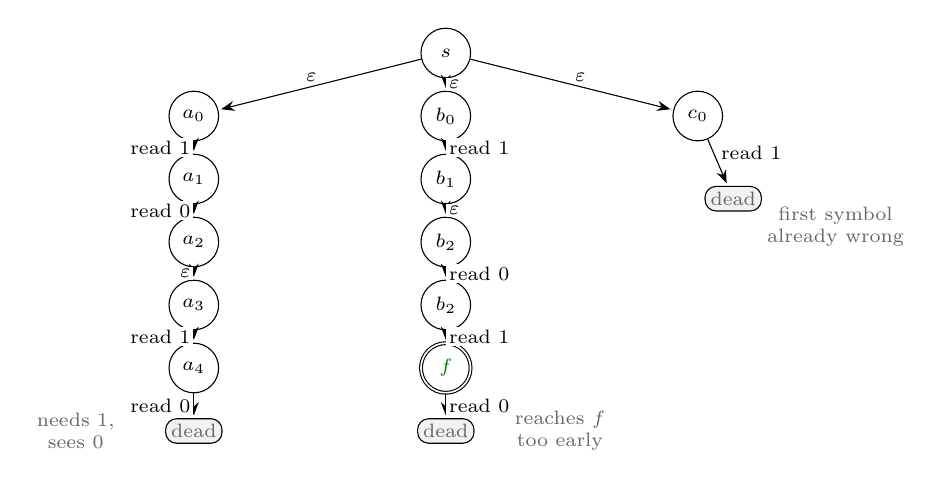
\begin{tikzpicture}[
  ->,>=Stealth,
  every node/.style={font=\scriptsize},
  st/.style={draw,circle,minimum size=6.3mm,inner sep=1pt},
  acc/.style={st,double,text=green!50!black},
  dead/.style={draw,rounded corners,fill=black!5,text=gray!80!black,inner sep=2pt},
  lab/.style={fill=white,inner sep=1pt,font=\scriptsize}
]

\node[st] (s) at (0,0) {$s$};

\node[st] (a0) at (-3.2,-0.8) {$a_0$};
\node[st] (b0) at (0,-0.8) {$b_0$};
\node[st] (c0) at (3.2,-0.8) {$c_0$};

\node[st] (a1) at (-3.2,-1.6) {$a_1$};
\node[st] (b1) at (0,-1.6) {$b_1$};
\node[dead] (cd) at (3.65,-1.85) {dead};

\node[st] (a2) at (-3.2,-2.4) {$a_2$};
\node[st] (b2e) at (0,-2.4) {$b_2$};

\node[st] (a3) at (-3.2,-3.2) {$a_3$};
\node[st] (b2) at (0,-3.2) {$b_2$};

\node[st] (a4) at (-3.2,-4.0) {$a_4$};
\node[acc] (fearly) at (0,-4.0) {$f$};

\node[dead] (ad) at (-3.2,-4.8) {dead};
\node[dead] (fd) at (0,-4.8) {dead};

\draw (s) -- node[lab,above left] {$\eps$} (a0);
\draw (s) -- node[lab,right] {$\eps$} (b0);
\draw (s) -- node[lab,above right] {$\eps$} (c0);

\draw (a0) -- node[lab,left] {read \(1\)} (a1);
\draw (b0) -- node[lab,right] {read \(1\)} (b1);
\draw (c0) -- node[lab,above right] {read \(1\)} (cd);

\draw (a1) -- node[lab,left] {read \(0\)} (a2);
\draw (b1) -- node[lab,right] {$\eps$} (b2e);

\draw (a2) -- node[lab,left] {$\eps$} (a3);
\draw (b2e) -- node[lab,right] {read \(0\)} (b2);

\draw (a3) -- node[lab,left] {read \(1\)} (a4);
\draw (b2) -- node[lab,right] {read \(1\)} (fearly);

\draw (a4) -- node[lab,left] {read \(0\)} (ad);
\draw (fearly) -- node[lab,right] {read \(0\)} (fd);

\node[text=gray!80!black,align=center] at (4.95,-2.2)
  {first symbol\\already wrong};
\node[text=gray!80!black,align=center] at (-4.7,-4.8)
  {needs \(1\),\\sees \(0\)};
\node[text=gray!80!black,align=center] at (1.45,-4.8)
  {reaches \(f\)\\too early};

\end{tikzpicture}
\end{center}

\vspace{0.2em}
Every branch either dies, or reaches an accepting state before the input is finished and then dies on the remaining symbol.

\end{frame}

%------------------------------------------------
\begin{frame}{Epsilon-Closure}

To remove \(\eps\)-transitions, we need one definition.

\vspace{0.8em}

The \textbf{epsilon-closure} of a state \(q\), denoted \(E(q)\), is:

\[
E(q)=\{r\in Q: r\text{ is reachable from }q\text{ using zero or more }\eps\text{-transitions}\}.
\]

\vspace{0.8em}

We include \(q\) itself:\(\quad
q\in E(q).
\)

\vspace{0.8em}

For a set \(S\subseteq Q\), define

\[
E(S)=\bigcup_{q\in S}E(q).
\]

\end{frame}

%------------------------------------------------
\begin{frame}{Removing Epsilon Transitions}

Every epsilon-NFA can be converted into an ordinary NFA.

\vspace{0.8em}

Let \(
M=(Q,\Sigma,\delta,q_0,F)
\) be an epsilon-NFA. 

We build \(
M'=(Q,\Sigma,\delta',q_0,F')
\) with no \(\eps\)-transitions.

\vspace{0.8em}

For each \(q\in Q\) and \(a\in\Sigma\), define

\[
\delta'(q,a)
=
E\left(\bigcup_{r\in E(q)}\delta(r,a)\right).
\]

\vspace{0.5em}

This says: take free moves, read \(a\), then take free moves again.

\end{frame}

%------------------------------------------------
\begin{frame}{Accepting States After Removing \(\eps\)}

We also update the accepting states.

\vspace{0.8em}

Define

\[
F'=\{q\in Q: E(q)\cap F\neq \emptyset\}.
\]

\vspace{0.8em}

Why?

\pause

If a state \(q\) can reach an accepting state using only \(\eps\)-moves, then \(q\) should be accepting in the new NFA.

\vspace{0.8em}

This handles the case where the epsilon-NFA accepts after the input has already been consumed.

\end{frame}

%------------------------------------------------
\begin{frame}{Why Epsilon Elimination Is Correct}

\small
The formula
\[
\delta'(q,a)
=
E\left(\bigcup_{r\in E(q)}\delta(r,a)\right)
\]
compresses one full block of behavior:

\[
\eps^*
\quad\text{then read }a\quad
\text{then }\eps^*.
\]

\vspace{0.7em}
So every one-symbol transition in \(M'\) represents a real path in the original epsilon-NFA.

\vspace{0.7em}
Conversely, every accepting computation in the epsilon-NFA can be broken into such blocks, one block for each real input symbol.

\vspace{0.7em}
The accepting-state update
\[
F'=\{q:E(q)\cap F\neq\emptyset\}
\]
handles final free \(\eps\)-moves after the input is finished.

\end{frame}

%------------------------------------------------
\begin{frame}{Proof Sketch: Same Language After Removing \(\eps\)}

\small
We show both inclusions.

\vspace{0.5em}
\textbf{If \(M'\) accepts \(w\):}
each transition of \(M'\) can be expanded into
\[
\eps^*\, a\, \eps^*
\]
inside \(M\). Expanding all transitions gives an accepting computation of \(M\).

\vspace{0.7em}
\textbf{If \(M\) accepts \(w\):}
take its accepting path and group it around the real input symbols:
\[
\eps^* a_1 \eps^* a_2 \eps^* \cdots a_k \eps^*.
\]
Each group is simulated by one transition of \(M'\). Final \(\eps\)-moves are handled by \(F'\).

\vspace{0.7em}
Therefore, \(L(M)=L(M')\).

\end{frame}

%------------------------------------------------
\begin{frame}{Example: An Epsilon-NFA over \(\{0,1\}\)}

Let
\[
Q=\{q_0,q_1,q_2,q_3,q_4\},
\qquad
\Sigma=\{0,1\},
\qquad
F=\{q_4\}.
\]

\begin{center}
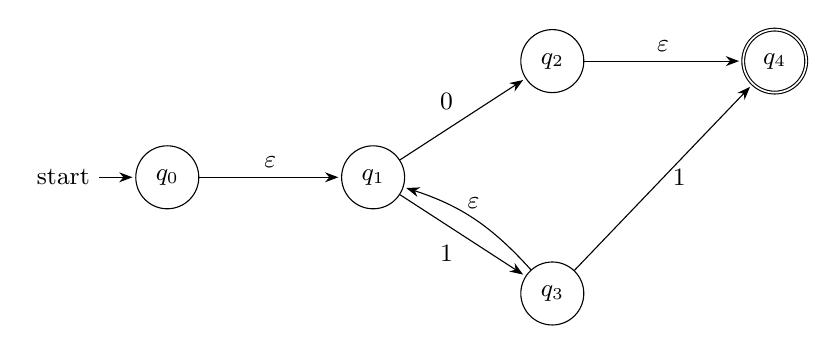
\begin{tikzpicture}[
  ->,>=Stealth,shorten >=1pt,
  node distance=2.0cm,
  every state/.style={minimum size=8mm},
  every node/.style={font=\small}
]

\node[state,initial] (q0) {$q_0$};
\node[state,right=1.8cm of q0] (q1) {$q_1$};
\node[state,above right=0.9cm and 1.7cm of q1] (q2) {$q_2$};
\node[state,below right=0.9cm and 1.7cm of q1] (q3) {$q_3$};
\node[state,accepting,right=2.0cm of q2] (q4) {$q_4$};

\path
(q0) edge node[above] {$\eps$} (q1)

(q1) edge node[above left] {$0$} (q2)
(q1) edge node[below left] {$1$} (q3)

(q2) edge node[above] {$\eps$} (q4)

(q3) edge[bend right=15] node[above] {$\eps$} (q1)
(q3) edge node[right] {$1$} (q4);

\end{tikzpicture}
\end{center}

\vspace{0.4em}

All missing transitions go to \(\emptyset\).

\end{frame}

%------------------------------------------------
\begin{frame}{Step 1: Compute Epsilon-Closures}

For the epsilon-NFA above:

\vspace{0.5em}

\begin{center}
\begin{tabular}{l|l}
\toprule
\textbf{State} & \textbf{Epsilon-closure}\\
\midrule
$q_0$ & $E(q_0)=\{q_0,q_1\}$\\
$q_1$ & $E(q_1)=\{q_1\}$\\
$q_2$ & $E(q_2)=\{q_2,q_4\}$\\
$q_3$ & $E(q_3)=\{q_3,q_1\}$\\
$q_4$ & $E(q_4)=\{q_4\}$\\
\bottomrule
\end{tabular}
\end{center}

\vspace{0.8em}

Notice:

\[
q_2\in F'
\]

because \(q_2\) can reach the accepting state \(q_4\) using only an \(\eps\)-move.

\end{frame}

%------------------------------------------------
\begin{frame}{Step 2: New Accepting States}

Original accepting states: \(
F=\{q_4\}.
\)

\vspace{0.8em}

After removing \(\eps\)-transitions:

\[
F'=\{q\in Q:E(q)\cap F\neq\emptyset\}.
\]

\vspace{0.8em}

From the closure table:

\[
E(q_2)=\{q_2,q_4\},
\qquad
E(q_4)=\{q_4\}.
\]

Therefore,

\[
F'=\{q_2,q_4\}.
\]

\end{frame}

%------------------------------------------------
\begin{frame}{Step 3: New Transition Table}

The converted NFA has no \(\eps\)-transitions.

\[
\delta'(q,a)
=
E\left(\bigcup_{r\in E(q)}\delta(r,a)\right).
\]

\vspace{0.5em}

\begin{center}
\begin{tabular}{c|cc}
\toprule
\textbf{State} & \textbf{on \(0\)} & \textbf{on \(1\)}\\
\midrule
$q_0$ & $\{q_2,q_4\}$ & $\{q_3,q_1\}$\\
$q_1$ & $\{q_2,q_4\}$ & $\{q_3,q_1\}$\\
$q_2$ & $\emptyset$ & $\emptyset$\\
$q_3$ & $\{q_2,q_4\}$ & $\{q_4,q_3,q_1\}$\\
$q_4$ & $\emptyset$ & $\emptyset$\\
\bottomrule
\end{tabular}
\end{center}

\vspace{0.4em}

Accepting states in the new NFA: \(\{q_2,q_4\}\).

\end{frame}

%------------------------------------------------
\begin{frame}{One Entry Explained}

\textit{\textbf{Question:} Why is} \(
\delta'(q_0,0)=\{q_2,q_4\}?
\)

\vspace{0.7em}

Start with the epsilon-closure. \(
E(q_0)=\{q_0,q_1\}.
\)

Then read \(0\):

\[
\delta(q_0,0)\cup\delta(q_1,0)
=
\emptyset\cup\{q_2\}
=
\{q_2\}.
\]

Then take epsilon-closure again:

\[
E(\{q_2\})=\{q_2,q_4\}.
\]

So

\[
\delta'(q_0,0)=\{q_2,q_4\}.
\]

\end{frame}


%------------------------------------------------
\begin{frame}{What This Means}

Epsilon transitions do not add new language-recognition power.

\vspace{0.8em}

They only make constructions cleaner.

\[
\text{epsilon-NFA}
\quad\Longleftrightarrow\quad
\text{NFA without epsilon transitions}
\]

\vspace{0.8em}

\pause

So we are free to use \(\eps\)-transitions when they make the design simpler.


\end{frame}

%------------------------------------------------
\begin{frame}{A Note on Terminology}

Different books use slightly different conventions.

\vspace{0.8em}

In Sipser's textbook, an \textbf{NFA} is allowed to have \(\eps\)-transitions.

\vspace{0.8em}

From now on, we will follow that convention:

\begin{center}
\textbf{When we say NFA, we allow \(\eps\)-transitions unless stated otherwise.}
\end{center}

\vspace{0.8em}

If we need to forbid them, we will explicitly say ``NFA without \(\eps\)-transitions.''

\end{frame}

%================================================
\section{Lecture 4E: Equivalence of DFA and NFA}

%------------------------------------------------
\begin{frame}{Machine Equivalence}

\textbf{Definition:} Two machines are equivalent if and only if they recognize the same language.

\vspace{1em}

We already know that every DFA is automatically an NFA. 

\pause
\vspace{1em}

\textbf{The surprising part:} 
Every NFA has an equivalent DFA.

\vspace{1em}

This means that adding nondeterminism does \textbf{not} increase the theoretical power of finite automata. They still recognize exactly the same set of languages, namely \textbf{the regular languages}.

\end{frame}

%------------------------------------------------
\begin{frame}{The Subset Construction (Idea)}

How can a deterministic machine simulate a nondeterministic one?

\vspace{1em}

\begin{itemize}
\item An NFA can be in multiple states at once across different branches of computation.
\item A DFA can only be in exactly one state.
\item \textbf{Solution:} Make the DFA's states represent \textit{sets} of NFA states!
\end{itemize}

\vspace{1em}

\pause
If the NFA has $Q$ as its set of states, the equivalent DFA will use the powerset $\powset{Q}$ as its states. 

\vspace{0.5em}

If $|Q| = n$, the DFA will have up to $2^n$ states.

\vspace{1em}
\textbf{Note:} We already showed that any NFA with $\epsilon$-transitions can be converted to one without them. Therefore, for this proof, we assume our starting NFA has no $\epsilon$-transitions.

\end{frame}

%------------------------------------------------
\begin{frame}{Formal Construction}

Let $N = (Q, \Sigma, \delta, q_0, F)$ be an NFA without $\epsilon$-transitions. 

We construct an equivalent DFA $M = (Q', \Sigma, \delta', q'_0, F')$ as follows:

\vspace{1em}

\begin{enumerate}
\item \textbf{States:} $Q' = \powset{Q}$.
\item \textbf{Start state:} $q'_0 = \{q_0\} \qquad$
(The set containing only the NFA start state).
\item \textbf{Accepting states:} 
\[
F' = \{ R \in Q' \mid R \cap F \neq \emptyset \}
\]
(Any subset containing at least one NFA accepting state).
\item \textbf{Transition function:} For any $R \in Q'$ and $a \in \Sigma$:
\[
\delta'(R, a) = \bigcup_{r \in R} \delta(r, a)
\]
\end{enumerate}

\end{frame}

%------------------------------------------------
\begin{frame}{Why the Subset Construction Is Correct}

\small
The key invariant is:

\[
\text{After reading }w,\text{ the DFA is in exactly the set of NFA states reachable after reading }w.
\]

\vspace{0.8em}
Base case:
\[
w=\eps.
\]
The DFA starts in \(\{q_0\}\), which is exactly where the NFA can be before reading input.

\vspace{0.8em}
Inductive step:
if the current set is \(R\), then after reading \(a\), the NFA may move from any state \(r\in R\) to any state in \(\delta(r,a)\).

\vspace{0.5em}
That is exactly:
\[
\delta'(R,a)=\bigcup_{r\in R}\delta(r,a).
\]

\end{frame}

%------------------------------------------------
\begin{frame}{Proof Sketch: Same Language After Subset Construction}

\small
By the invariant, after reading any string \(w\), the DFA state is the set of all NFA states reachable after reading \(w\).

\vspace{0.8em}
The NFA accepts \(w\) iff at least one reachable state is accepting:
\[
\text{reachable set}\cap F\neq\emptyset.
\]

\vspace{0.8em}
The subset-construction DFA declares exactly those subsets accepting:
\[
F'=\{R\subseteq Q:R\cap F\neq\emptyset\}.
\]

\vspace{0.8em}
Therefore, for every input \(w\),
\[
w\in L(N)\quad\Longleftrightarrow\quad w\in L(M).
\]

\end{frame}

%------------------------------------------------
\begin{frame}{Worked Example}

Let's convert an NFA that recognizes strings containing the substring $aba$.

\vspace{1em}

\begin{center}
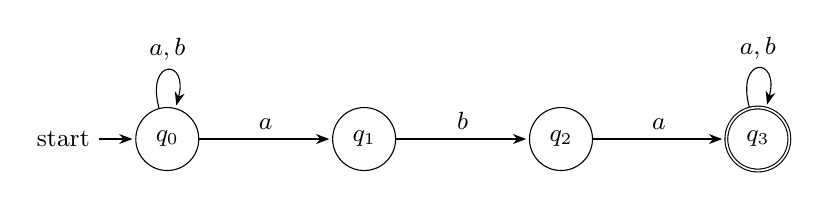
\begin{tikzpicture}[
  ->,>=Stealth,shorten >=1pt,
  node distance=2.5cm,
  every state/.style={minimum size=8mm},
  every node/.style={font=\small}
]

\node[state,initial] (q0) {$q_0$};
\node[state,right of=q0] (q1) {$q_1$};
\node[state,right of=q1] (q2) {$q_2$};
\node[state,accepting,right of=q2] (q3) {$q_3$};

\path
(q0) edge[loop above] node {$a,b$} ()
(q0) edge node[above] {$a$} (q1)
(q1) edge node[above] {$b$} (q2)
(q2) edge node[above] {$a$} (q3)
(q3) edge[loop above] node {$a,b$} ();

\end{tikzpicture}
\end{center}

\vspace{1em}

$Q = \{q_0, q_1, q_2, q_3\}$.

The theoretical equivalent DFA has states in $\powset{Q}$, meaning $2^4 = 16$ possible states. 

\pause
\vspace{0.5em}
\textbf{Good news:} We only need to construct the states that are actually \textit{reachable} from the start state.

\end{frame}

%------------------------------------------------
\begin{frame}{Step-by-Step Conversion: Setup and Initial States}

\textbf{1. Start State:} \\
The DFA start state is simply the set containing the NFA start state: $A = \{q_0\}$.

\vspace{1em}
\pause

\textbf{2. Transitions from $A = \{q_0\}$:}
\begin{itemize}
\item On $a$: $\delta(q_0, a) = \{q_0, q_1\}$. \quad \textrightarrow\ New state $B = \{q_0, q_1\}$.
\item On $b$: $\delta(q_0, b) = \{q_0\}$. \quad \quad \ \ \ \textrightarrow\ Back to $A$.
\end{itemize}

\vspace{1em}
\pause

\textbf{3. Transitions from $B = \{q_0, q_1\}$:}
\begin{itemize}
\item On $a$: $\delta(q_0, a) \cup \delta(q_1, a) = \{q_0, q_1\} \cup \emptyset = \{q_0, q_1\}$. \quad \textrightarrow\ Back to $B$.
\item On $b$: $\delta(q_0, b) \cup \delta(q_1, b) = \{q_0\} \cup \{q_2\} = \{q_0, q_2\}$. \quad \textrightarrow\ New state $C = \{q_0, q_2\}$.
\end{itemize}

\end{frame}

%------------------------------------------------
\begin{frame}{Step-by-Step Conversion: The Domino Effect}

\textbf{4. Transitions from $C = \{q_0, q_2\}$:}
\begin{itemize}
\item On $a$: $\delta(q_0, a) \cup \delta(q_2, a) = \{q_0, q_1\} \cup \{q_3\} = \{q_0, q_1, q_3\}$. \textrightarrow\ New state $D$.
\item On $b$: $\delta(q_0, b) \cup \delta(q_2, b) = \{q_0\} \cup \emptyset = \{q_0\}$. \quad \quad \quad \quad \ \ \, \textrightarrow\ Back to $A$.
\end{itemize}

\vspace{1em}
\pause

\textbf{5. Transitions from $D = \{q_0, q_1, q_3\}$:} \\
\textit{(Note: Since $q_3 \in D$, $D$ is an accepting state!)}
\begin{itemize}
\item On $a$: $\{q_0, q_1\} \cup \emptyset \cup \{q_3\} = \{q_0, q_1, q_3\}$. \quad \quad \quad \ \ \, \textrightarrow\ Back to $D$.
\item On $b$: $\{q_0\} \cup \{q_2\} \cup \{q_3\} = \{q_0, q_2, q_3\}$. \quad \quad \quad \ \ \, \textrightarrow\ New state $E$.
\end{itemize}

\vspace{1em}
\pause

\textit{Wait, another state? Let's keep going...}

\end{frame}

%------------------------------------------------
\begin{frame}{Step-by-Step Conversion: Reaching Closure}

\textbf{6. Transitions from $E = \{q_0, q_2, q_3\}$:} \textit{(Accepting)}
\begin{itemize}
\item On $a$: $\{q_0, q_1\} \cup \{q_3\} \cup \{q_3\} = \{q_0, q_1, q_3\}$. \quad \quad \, \textrightarrow\ Goes to $D$.
\item On $b$: $\{q_0\} \cup \emptyset \cup \{q_3\} = \{q_0, q_3\}$. \quad \quad \quad \quad \quad \textrightarrow\ New state $F$.
\end{itemize}

\vspace{1em}
\pause

\textbf{7. Transitions from $F = \{q_0, q_3\}$:} \textit{(Accepting)}
\begin{itemize}
\item On $a$: $\{q_0, q_1\} \cup \{q_3\} = \{q_0, q_1, q_3\}$. \quad \quad \quad \quad \quad \textrightarrow\ Goes to $D$.
\item On $b$: $\{q_0\} \cup \{q_3\} = \{q_0, q_3\}$. \quad \quad \quad \quad \quad \quad \quad \, \textrightarrow\ Back to $F$.
\end{itemize}

\vspace{1em}
\pause

\textbf{Done!} No new states were generated. Out of 16 possible subsets, only 6 are reachable from the start state. 

\end{frame}

%------------------------------------------------
\begin{frame}{The Equivalent DFA}

Here is the deterministic machine we just built. It elegantly tracks the longest matching prefix of the target substring $aba$.

\vspace{1em}

\begin{center}
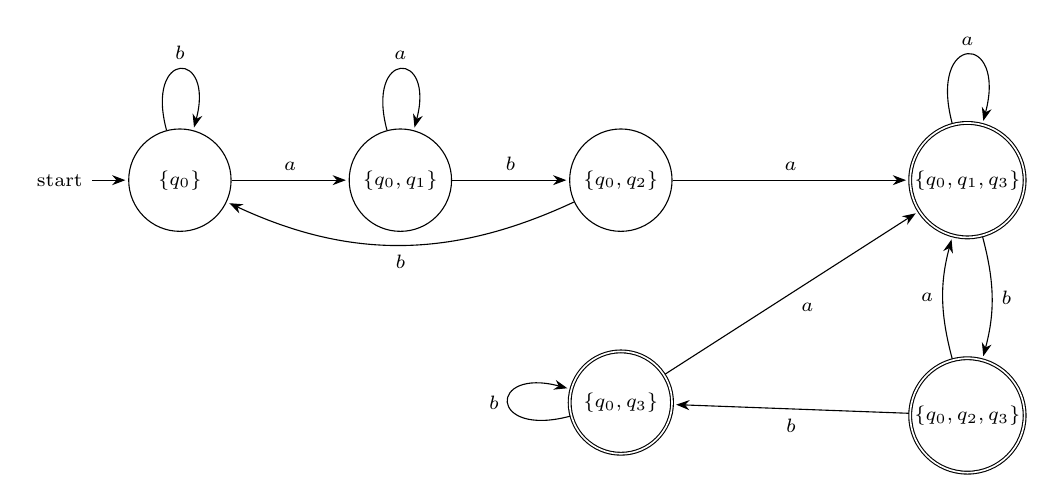
\begin{tikzpicture}[
  ->,>=Stealth,shorten >=1pt,
  node distance=2.8cm,
  every state/.style={minimum size=13mm, inner sep=1pt},
  every node/.style={font=\scriptsize}
]

% States
\node[state,initial] (A) {$\{q_0\}$};
\node[state,right of=A] (B) {$\{q_0,q_1\}$};
\node[state,right of=B] (C) {$\{q_0,q_2\}$};
\node[state,accepting,right=3cm of C] (D) {$\{q_0,q_1,q_3\}$};
\node[state,accepting,below=1.5cm of D] (E) {$\{q_0,q_2,q_3\}$};
\node[state,accepting,below=1.5cm of C] (F) {$\{q_0,q_3\}$};

% Transitions
\path
(A) edge[loop above] node {$b$} ()
(A) edge node[above] {$a$} (B)

(B) edge[loop above] node {$a$} ()
(B) edge node[above] {$b$} (C)

(C) edge node[above] {$a$} (D)
(C) edge[bend left=25] node[below] {$b$} (A)

(D) edge[loop above] node {$a$} ()
(D) edge[bend left=15] node[right] {$b$} (E)

(E) edge[bend left=15] node[left] {$a$} (D)
(E) edge node[below] {$b$} (F)

(F) edge[loop left] node {$b$} ()
(F) edge node[below right] {$a$} (D);

\end{tikzpicture}
\end{center}

\end{frame}

%------------------------------------------------
\begin{frame}{Comments about the Conversion}
    There can be smaller equivalent DFAs than the ones we can find using this explicit construction. 
    
    \medskip 
    However, we need a generalized procedure to show that every language recognized by some NFA can also be recognized by some DFA.
\end{frame}
\end{document}

